\documentclass[11pt,a4paper]{article}

% ===== PACKAGES =====
\usepackage[utf8]{inputenc}
\usepackage[T1]{fontenc}
\usepackage{amsmath,amssymb,amsthm}
\usepackage{mathtools}
\usepackage{bm}
\usepackage{geometry}
\usepackage{graphicx}
\usepackage{float}
\usepackage{booktabs}
\usepackage{array}
\usepackage{enumitem}
\usepackage{xcolor}
\usepackage{hyperref}
\usepackage{fancyhdr}
\usepackage{titlesec}
\usepackage{tcolorbox}
\usepackage{siunitx}
\usepackage{caption}
\usepackage{subcaption}

% ===== PAGE SETUP =====
\geometry{margin=1in}
\setlength{\parindent}{0pt}
\setlength{\parskip}{0.5em}

% ===== COLORS =====
\definecolor{primaryblue}{RGB}{59, 130, 246}
\definecolor{accentorange}{RGB}{249, 115, 22}
\definecolor{successgreen}{RGB}{34, 197, 94}
\definecolor{warningyellow}{RGB}{234, 179, 8}
\definecolor{darkbg}{RGB}{17, 24, 39}

% ===== HYPERREF SETUP =====
\hypersetup{
    colorlinks=true,
    linkcolor=primaryblue,
    urlcolor=primaryblue,
    citecolor=primaryblue
}

% ===== HEADER/FOOTER =====
\pagestyle{fancy}
\fancyhf{}
\fancyhead[L]{\textsc{Sentinal Nano S1}}
\fancyhead[R]{\textsc{Conrad Challenge 2026}}
\fancyfoot[C]{\thepage}
\renewcommand{\headrulewidth}{0.4pt}

% ===== CUSTOM BOXES =====
\tcbuselibrary{skins,breakable}

\newtcolorbox{mathbox}[1][]{
    colback=primaryblue!5,
    colframe=primaryblue!50,
    fonttitle=\bfseries,
    title=#1,
    breakable
}

\newtcolorbox{warningbox}[1][]{
    colback=warningyellow!10,
    colframe=warningyellow!70,
    fonttitle=\bfseries,
    title=#1,
    breakable
}

\newtcolorbox{notebox}[1][]{
    colback=successgreen!5,
    colframe=successgreen!50,
    fonttitle=\bfseries,
    title=#1,
    breakable
}

% ===== TITLE =====
\title{
    \vspace{-1cm}
    {\Large\textsc{Conrad Challenge 2026}}\\[0.5em]
    {\Huge\textbf{Sentinal Nano S1}}\\[0.3em]
    {\large Indoor Positioning System for Firefighters}\\[0.3em]
    {\normalsize UWB Multilateration with ML Bias Correction}
}
\author{
    Naitik Gupta \and Julian Juan \and Ming Ying \and Ayush Iyer \and Gavyn Liu
}
\date{}

% ===== DOCUMENT =====
\begin{document}

\maketitle
\thispagestyle{empty}

\begin{abstract}
Every year, firefighters lose their lives due to disorientation inside burning structures. GPS signals cannot penetrate buildings, leaving incident commanders with no reliable way to track their teams indoors. \textbf{Sentinal Nano S1} is a wearable Ultra-Wideband (UWB) positioning system that computes real-time 3D coordinates using geometric multilateration. The system deploys fixed UWB anchors at known coordinates, with each firefighter wearing a tag that ranges to visible anchors. Position is computed via weighted nonlinear least squares, with an ML model correcting for Non-Line-of-Sight (NLOS) bias caused by wall reflections.
\end{abstract}

\tableofcontents
\newpage

% =============================================================================
\section{Problem Statement}
% =============================================================================

Firefighter disorientation in burning structures is a leading cause of line-of-duty deaths. The challenges include:

\begin{itemize}[leftmargin=2em]
    \item \textbf{GPS denial}: Satellite signals cannot penetrate building interiors
    \item \textbf{Visual impairment}: Smoke reduces visibility to near-zero
    \item \textbf{Communication breakdown}: Radio signals may be unreliable
    \item \textbf{Structural changes}: Fire can alter building layout during operations
\end{itemize}

Incident commanders need real-time position data to:
\begin{enumerate}
    \item Track team locations on a floor plan
    \item Coordinate search patterns
    \item Guide rescue operations if a firefighter becomes trapped
    \item Account for all personnel during evacuation
\end{enumerate}

% =============================================================================
\section{System Overview}
% =============================================================================

The Sentinal Nano S1 system consists of four main components:

\begin{enumerate}
    \item \textbf{Wearable Tag}: Worn by each firefighter, performs UWB ranging
    \item \textbf{Fixed Anchors}: 4--6 units deployed around the structure with known positions
    \item \textbf{Base Station}: Receives range data, computes positions, displays on map
    \item \textbf{Drone Anchor} (optional): Mobile anchor to improve geometry in obstructed areas
\end{enumerate}

\subsection{Algorithm Pipeline}

The real-time position computation follows this pipeline:

\begin{enumerate}
    \item \textbf{Collect UWB ranges} $d_i$ from visible anchors
    \item \textbf{Apply ML correction}: $d_{\text{corr}} = d_i - \hat{\Delta}_i$, compute weight
    \item \textbf{Solve multilateration}: $(x, y, z)$ via weighted least squares
    \item \textbf{Tracking filter}: Predict $\rightarrow$ correct with IMU
    \item \textbf{Output position}: $(x, y, z, \text{confidence}, \text{timestamp})$
\end{enumerate}

% =============================================================================
\section{Hardware Design}
% =============================================================================

\subsection{Wearable Tag (1 per firefighter)}

\begin{table}[H]
\centering
\begin{tabular}{@{}lll@{}}
\toprule
\textbf{Component} & \textbf{Part Number} & \textbf{Function} \\
\midrule
Main Controller & Raspberry Pi Pico 2 W & Dual-core ARM Cortex-M33, WiFi/BLE \\
UWB Module & DWM3000 & Time-of-flight ranging, IEEE 802.15.4z \\
Boost Converter & TPS61022 & 3.7V $\rightarrow$ stable 3.3V rail \\
Charger IC & TP4056 & Li-ion charging via USB-C \\
Battery & 18650 Li-ion & $\sim$12h runtime \\
PCB & 2-layer & RF-aware layout with keep-out zones \\
\bottomrule
\end{tabular}
\caption{Wearable tag bill of materials}
\end{table}

\textbf{Optional Sensors:}
\begin{itemize}
    \item IMU (BMI270) -- 6-axis accelerometer/gyroscope for dead reckoning
    \item Barometer -- Altitude estimation for multi-floor buildings
\end{itemize}

\subsection{PCB Design}

The tag PCB integrates all components on a compact 2-layer board with careful RF layout considerations.

\begin{figure}[H]
    \centering
    \begin{subfigure}[b]{0.48\textwidth}
        \centering
        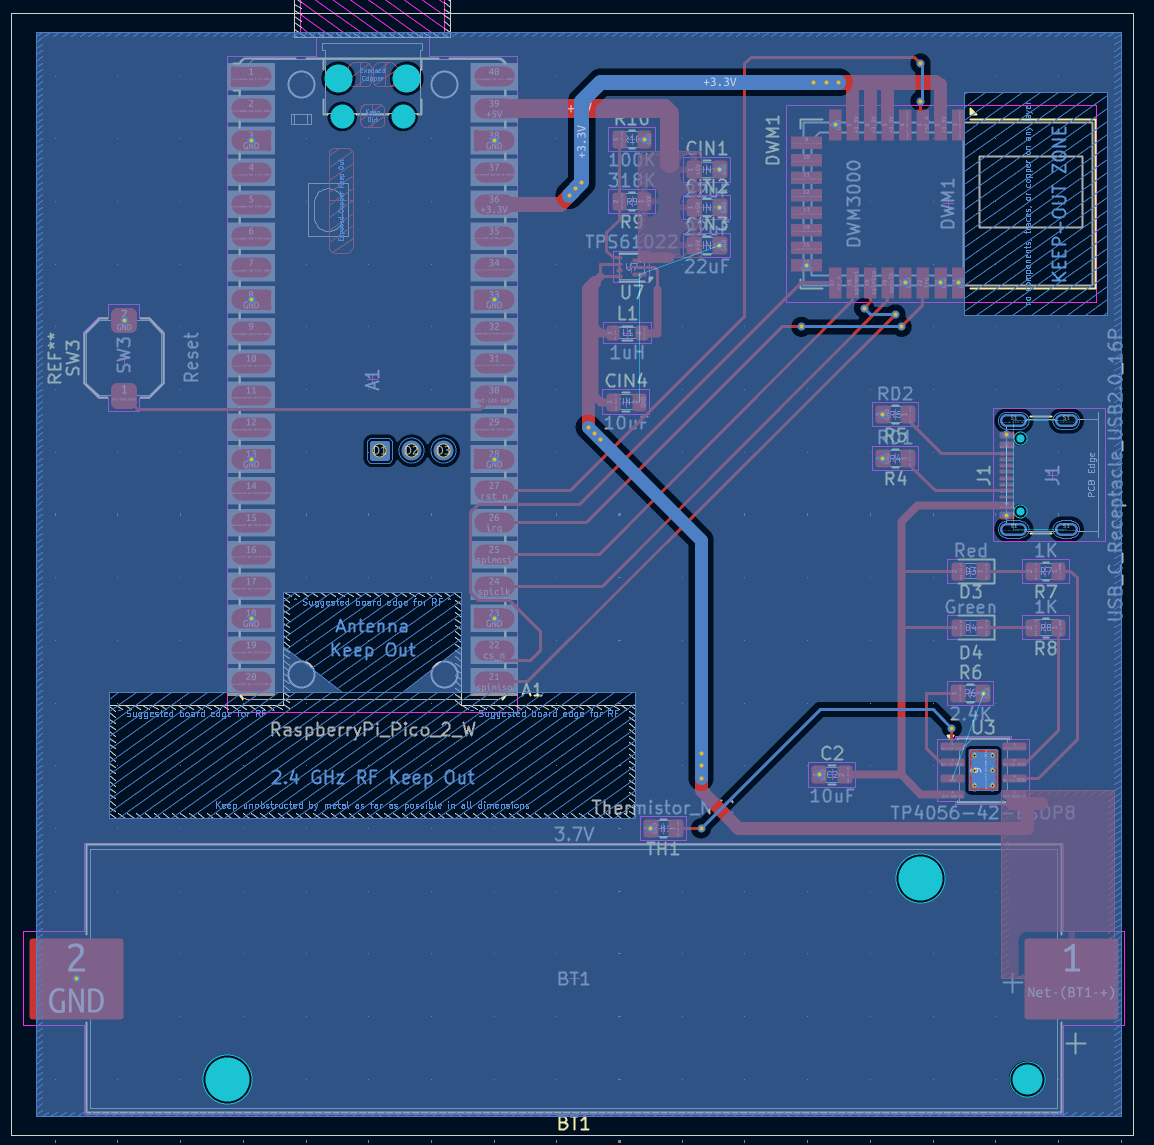
\includegraphics[width=\textwidth]{86.png}
        \caption{PCB layout showing component placement and routing}
        \label{fig:pcb_layout}
    \end{subfigure}
    \hfill
    \begin{subfigure}[b]{0.48\textwidth}
        \centering
        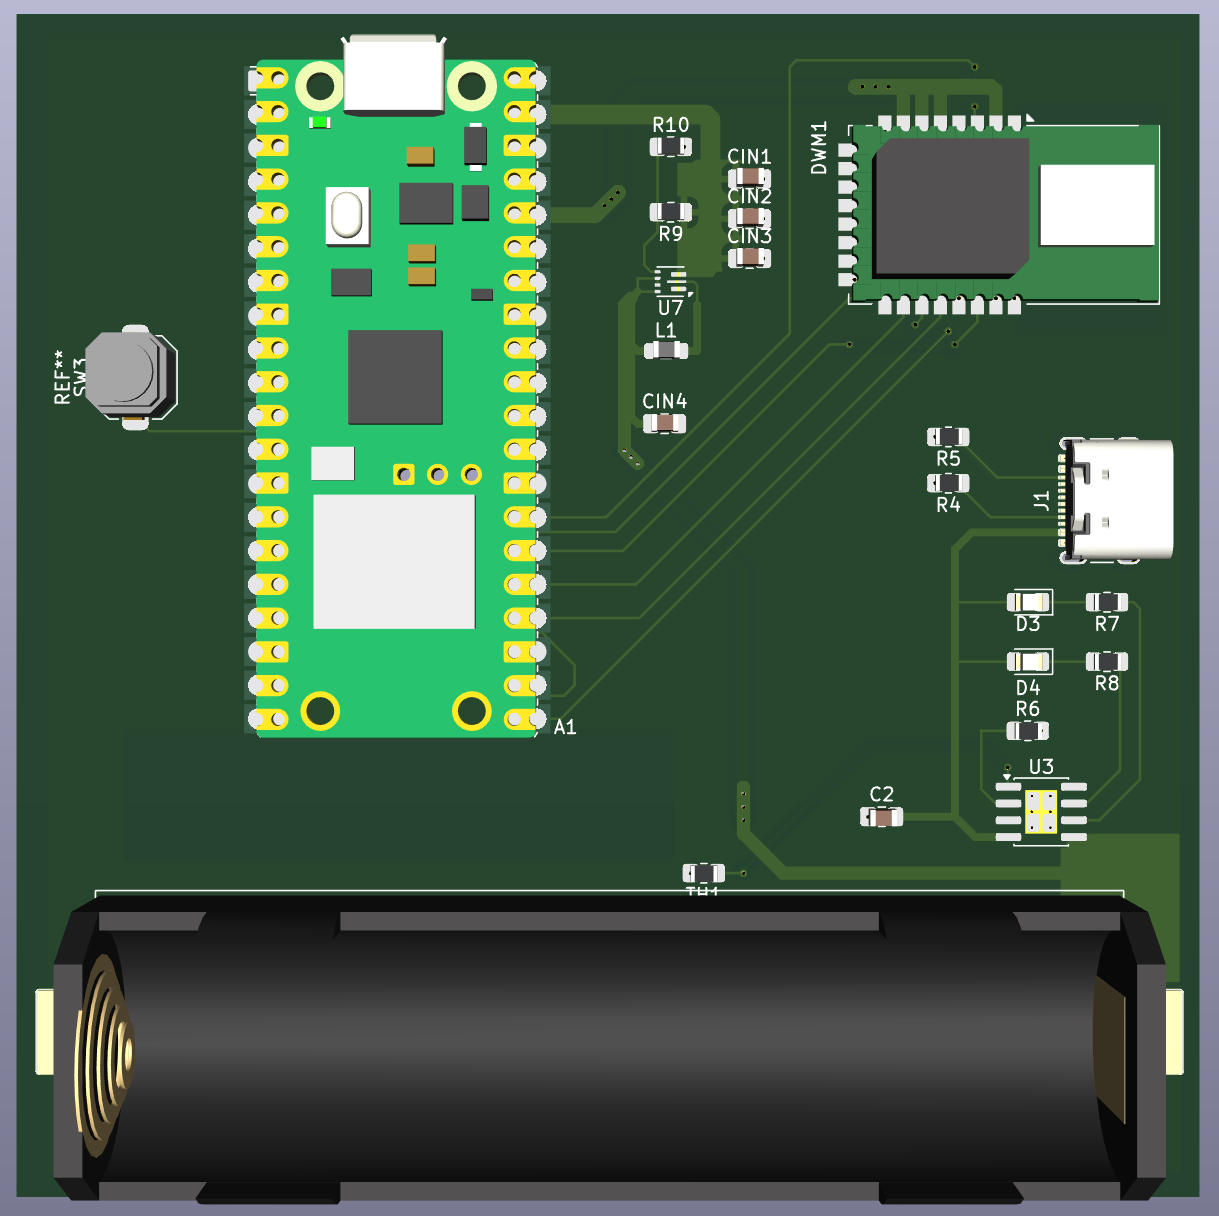
\includegraphics[width=\textwidth]{0.png}
        \caption{3D render of assembled PCB with 18650 battery}
        \label{fig:pcb_3d}
    \end{subfigure}
    \caption{Sentinal Nano S1 tag PCB design}
    \label{fig:pcb}
\end{figure}

Key design features:
\begin{itemize}
    \item \textbf{Antenna Keep-Out Zone}: Clear area around Pico 2 W antenna for 2.4 GHz WiFi/BLE
    \item \textbf{DWM3000 Keep-Out Zone}: Unobstructed area for UWB antenna performance
    \item \textbf{RF Routing}: Controlled impedance traces for RF signals
    \item \textbf{Power Planes}: Solid ground plane for noise reduction
    \item \textbf{Thermal Management}: Adequate copper pour for heat dissipation
\end{itemize}

\subsection{Fixed Anchors (4--6 units)}

\begin{itemize}
    \item Same electronics as tag (shared BOM reduces cost)
    \item Wall-powered or battery-operated
    \item Known surveyed position $(x_i, y_i, z_i)$
    \item Unique ID for identification
\end{itemize}

\subsection{Base Station}

\begin{itemize}
    \item \textbf{Demo mode}: USB tethered to laptop
    \item \textbf{Field mode}: LoRa wireless backhaul
    \item Runs position solver and displays map
\end{itemize}

\subsection{Drone Anchor (Optional)}

\begin{itemize}
    \item Mobile UWB anchor mounted on drone
    \item Position tracked via RTK-GPS when outside, visual odometry inside
    \item Provides additional range measurement from above
    \item Improves geometric dilution of precision (GDOP)
\end{itemize}

% =============================================================================
\section{Coordinate System and Geometry}
% =============================================================================

\subsection{Building Coordinate Frame}

We establish a local coordinate system:
\begin{itemize}
    \item Origin $O_B$ at a building corner (e.g., front-left at ground level)
    \item $+x$ axis along one wall
    \item $+y$ axis along perpendicular wall
    \item $+z$ axis pointing upward
\end{itemize}

No GPS or satellites required---purely local coordinate system.

\subsection{Anchor Surveying}

Each anchor position is measured using a laser distance meter:
\begin{equation}
    \mathbf{p}_i = \begin{bmatrix} x_i \\ y_i \\ z_i \end{bmatrix} \in \mathbb{R}^3, \quad i = 1, 2, 3, 4
\end{equation}

These coordinates are stored in a configuration file loaded at system startup.

\begin{warningbox}[Placement Requirements]
\begin{itemize}
    \item \textbf{Minimum}: 4 anchors for 3D positioning
    \item \textbf{Recommended}: 5--6 anchors for redundancy and outlier rejection
    \item \textbf{Height diversity}: Some anchors high, some low
    \item \textbf{Non-coplanar}: Anchors must not all lie in the same plane
\end{itemize}
\end{warningbox}

% =============================================================================
\section{Multilateration Mathematics}
% =============================================================================

\subsection{Problem Formulation}

Let the 4 anchors have known 3D positions:
\begin{equation}
    \mathbf{p}_i = \begin{bmatrix} x_i \\ y_i \\ z_i \end{bmatrix} \in \mathbb{R}^3, \quad i = 1, 2, 3, 4
\end{equation}

Let the measured ranges (from time-of-flight) be $r_i \geq 0$. The unknown tag position is:
\begin{equation}
    \mathbf{x} = \begin{bmatrix} x \\ y \\ z \end{bmatrix}
\end{equation}

\subsection{Sphere Intersection Model}

Each range measurement defines a sphere centered at the anchor:
\begin{equation}
    \|\mathbf{x} - \mathbf{p}_i\|^2 = r_i^2, \quad i = 1, 2, 3, 4
\end{equation}

Expanding:
\begin{equation}
    \mathbf{x}^\top \mathbf{x} - 2\mathbf{p}_i^\top \mathbf{x} + \mathbf{p}_i^\top \mathbf{p}_i = r_i^2
\end{equation}

\subsection{Linear System (Closed-Form Initialization)}

Subtracting the $i=1$ equation from $i = 2, 3, 4$ eliminates the quadratic term $\mathbf{x}^\top \mathbf{x}$:
\begin{equation}
    2(\mathbf{p}_i - \mathbf{p}_1)^\top \mathbf{x} = r_1^2 - r_i^2 + \|\mathbf{p}_i\|^2 - \|\mathbf{p}_1\|^2
\end{equation}

\begin{mathbox}[Matrix Form]
Define:
\begin{equation}
    \mathbf{A} = 2 \begin{bmatrix} 
        (\mathbf{p}_2 - \mathbf{p}_1)^\top \\
        (\mathbf{p}_3 - \mathbf{p}_1)^\top \\
        (\mathbf{p}_4 - \mathbf{p}_1)^\top 
    \end{bmatrix} \in \mathbb{R}^{3 \times 3}
\end{equation}

\begin{equation}
    \mathbf{b} = \begin{bmatrix}
        r_1^2 - r_2^2 + \|\mathbf{p}_2\|^2 - \|\mathbf{p}_1\|^2 \\
        r_1^2 - r_3^2 + \|\mathbf{p}_3\|^2 - \|\mathbf{p}_1\|^2 \\
        r_1^2 - r_4^2 + \|\mathbf{p}_4\|^2 - \|\mathbf{p}_1\|^2
    \end{bmatrix} \in \mathbb{R}^3
\end{equation}

Then:
\begin{equation}
    \mathbf{A}\mathbf{x} = \mathbf{b}
\end{equation}

If anchors are \textbf{not coplanar} ($\mathbf{A}$ is invertible), the unique solution is:
\begin{equation}
    \boxed{\mathbf{x}_0 = \mathbf{A}^{-1} \mathbf{b}}
\end{equation}
\end{mathbox}

\textbf{Degeneracy condition}: $\det(\mathbf{A}) = 0$ when anchors are coplanar or collinear, making the estimate unstable or non-unique.

\subsection{Nonlinear Least Squares (Optimal Estimator)}

With measurement noise, the four sphere equations won't intersect perfectly. We use nonlinear least squares on range residuals.

\subsubsection{Residual Definition}

\begin{equation}
    e_i(\mathbf{x}) = \|\mathbf{x} - \mathbf{p}_i\| - r_i, \quad i = 1, \dots, M
\end{equation}

\subsubsection{Objective Function}

\begin{mathbox}[Weighted Nonlinear Least Squares]
\begin{equation}
    \boxed{\min_{\mathbf{x}} \sum_{i=1}^{M} w_i \, e_i(\mathbf{x})^2}
\end{equation}
where $w_i = 1/\sigma_i^2$ is the weight (inverse variance) for each measurement.
\end{mathbox}

\subsubsection{Jacobian}

The Jacobian row for anchor $i$:
\begin{equation}
    \mathbf{J}_i(\mathbf{x}) = \frac{\partial e_i}{\partial \mathbf{x}} = \frac{(\mathbf{x} - \mathbf{p}_i)^\top}{\|\mathbf{x} - \mathbf{p}_i\|} \in \mathbb{R}^{1 \times 3}
\end{equation}

Stack all residuals and Jacobian rows:
\begin{equation}
    \mathbf{e} = \begin{bmatrix} e_1 \\ \vdots \\ e_M \end{bmatrix} \in \mathbb{R}^M, \quad
    \mathbf{J} = \begin{bmatrix} \mathbf{J}_1 \\ \vdots \\ \mathbf{J}_M \end{bmatrix} \in \mathbb{R}^{M \times 3}
\end{equation}

\subsubsection{Gauss-Newton Update}

\begin{mathbox}[Iterative Solution]
\begin{equation}
    \boxed{\Delta \mathbf{x} = -(\mathbf{J}^\top \mathbf{W} \mathbf{J})^{-1} \mathbf{J}^\top \mathbf{W} \mathbf{e}}
\end{equation}
\begin{equation}
    \mathbf{x} \leftarrow \mathbf{x} + \Delta \mathbf{x}
\end{equation}
where $\mathbf{W} = \text{diag}(w_1, \dots, w_M)$ is the weight matrix.
\end{mathbox}

For better convergence near the solution, use \textbf{Levenberg-Marquardt}:
\begin{equation}
    \Delta \mathbf{x} = -(\mathbf{J}^\top \mathbf{W} \mathbf{J} + \lambda \mathbf{I})^{-1} \mathbf{J}^\top \mathbf{W} \mathbf{e}
\end{equation}
where $\lambda > 0$ is a damping parameter.

\subsubsection{Weighted Least Squares (Linear, Overdetermined)}

With $M > 4$ anchors, the linear system is overdetermined. Use weighted least squares:
\begin{equation}
    \boxed{\mathbf{x} = (\mathbf{A}^\top \mathbf{W} \mathbf{A})^{-1} \mathbf{A}^\top \mathbf{W} \mathbf{b}}
\end{equation}

\subsection{Robust Estimation}

\begin{warningbox}[Outlier Handling]
A single bad NLOS measurement can corrupt the position estimate (``teleporting''). Use robust M-estimators:

\textbf{Huber weights}:
\begin{equation}
    w_i = \begin{cases}
        1 & \text{if } |e_i| \leq k \\
        k / |e_i| & \text{if } |e_i| > k
    \end{cases}
\end{equation}

\textbf{Tukey bisquare weights}:
\begin{equation}
    w_i = \begin{cases}
        \left(1 - (e_i/k)^2\right)^2 & \text{if } |e_i| \leq k \\
        0 & \text{if } |e_i| > k
    \end{cases}
\end{equation}

Iterate: solve $\rightarrow$ compute residuals $\rightarrow$ update weights $\rightarrow$ repeat.
\end{warningbox}

\subsection{Geometric Considerations}

\begin{notebox}[Key Points]
\begin{itemize}
    \item \textbf{Four anchors is the minimum} for 3D with absolute ranges; more anchors improve conditioning and enable outlier rejection
    \item \textbf{Good geometry matters}: Anchors spread in 3D (not coplanar) reduces Geometric Dilution of Precision (GDOP)
    \item \textbf{Two-solution ambiguity}: With only 3 anchors, intersection of 3 spheres can yield up to 2 points. The 4th anchor resolves this
\end{itemize}
\end{notebox}

% =============================================================================
\section{UWB Ranging Physics}
% =============================================================================

\subsection{Time-of-Flight Measurement}

UWB ranging uses Two-Way Ranging (TWR) to measure distance:
\begin{equation}
    d_i = \frac{c \cdot \Delta t}{2}
\end{equation}
where:
\begin{itemize}
    \item $c = 299{,}792{,}458$ m/s is the speed of light
    \item $\Delta t$ is the round-trip time
\end{itemize}

\subsection{Error Sources}

\begin{table}[H]
\centering
\begin{tabular}{@{}lll@{}}
\toprule
\textbf{Error Source} & \textbf{Magnitude} & \textbf{Mitigation} \\
\midrule
Clock drift & $\sim$1--10 cm & Two-way ranging cancels symmetric drift \\
Multipath & $\sim$10--100 cm & First-path detection algorithms \\
NLOS bias & $\sim$10--300 cm & ML bias correction \\
Antenna delay & $\sim$1--5 cm & Factory calibration \\
\bottomrule
\end{tabular}
\caption{UWB ranging error sources and mitigations}
\end{table}

% =============================================================================
\section{ML Bias Correction}
% =============================================================================

\subsection{Motivation}

Indoor ranging errors are often \textbf{systematic}---walls add consistent positive bias (signal travels longer path), not purely random noise. A trained model predicts this bias from signal features.

\subsection{Model Architecture}

\textbf{Input features}:
\begin{itemize}
    \item Measured distance $d_{\text{meas}}$
    \item Anchor ID (one-hot encoded)
    \item Received signal strength indicator (RSSI)
    \item First-path power
    \item Signal-to-noise ratio (SNR)
    \item Channel impulse response statistics
\end{itemize}

\textbf{Output}:
\begin{itemize}
    \item $\hat{b}$ --- predicted bias (meters)
    \item $\hat{\sigma}$ --- predicted uncertainty (meters)
\end{itemize}

\subsection{Runtime Correction}

\begin{mathbox}[Bias Correction]
\textbf{Corrected distance}:
\begin{equation}
    d_{\text{corr}} = d_{\text{meas}} - \hat{b}
\end{equation}

\textbf{Weight for multilateration}:
\begin{equation}
    w = \frac{1}{\max(\hat{\sigma}^2, \sigma_{\text{floor}}^2)}
\end{equation}
where $\sigma_{\text{floor}}$ prevents division by zero for high-confidence predictions.
\end{mathbox}

\subsection{Key Insight}

The ML model outputs \textbf{range corrections}, not positions directly. Position is computed geometrically via multilateration. This keeps the system:
\begin{itemize}
    \item \textbf{Interpretable}: Can inspect individual range corrections
    \item \textbf{Debuggable}: Geometry errors separate from ML errors
    \item \textbf{Robust}: Falls back to uncorrected ranges if model fails
\end{itemize}

% =============================================================================
\section{Training Data Collection}
% =============================================================================

\subsection{Ground Truth Method}

\begin{enumerate}
    \item Create taped floor grid with 0.5 m spacing
    \item Measure grid coordinates with laser distance meter
    \item Stand at each point for 3--5 seconds, log all ranges
    \item Record: timestamp, position, anchor ID, $d_{\text{meas}}$, signal features
\end{enumerate}

\subsection{Label Computation}

\begin{equation}
    d_{\text{true}} = \|\mathbf{p}_{\text{gt}} - \mathbf{a}_i\|
\end{equation}
\begin{equation}
    b_{\text{label}} = d_{\text{meas}} - d_{\text{true}}
\end{equation}

\subsection{Data Categories}

\begin{table}[H]
\centering
\begin{tabular}{@{}lll@{}}
\toprule
\textbf{Category} & \textbf{Description} & \textbf{Expected Bias} \\
\midrule
LOS & Tag and anchor in same room, clear sightline & $\sim$0--5 cm \\
NLOS (soft) & Signal through drywall/wood & $\sim$5--30 cm \\
NLOS (hard) & Signal through concrete/metal & $\sim$30--200 cm \\
\bottomrule
\end{tabular}
\caption{Training data categories}
\end{table}

\begin{notebox}[Train/Test Split]
Split by \textbf{room or hallway}, not random time samples. This proves the model generalizes to new environments, not just memorizes specific locations.
\end{notebox}

% =============================================================================
\section{Build Plan}
% =============================================================================

\subsection{Phase 1: Tag Bring-up (Foundation)}

\begin{itemize}
    \item[$\square$] Pico $\leftrightarrow$ DWM3000 SPI communication stable
    \item[$\square$] 2-way ranging verified in open space
    \item[$\square$] Logs: (timestamp, anchor\_id, $d_{\text{meas}}$, quality)
\end{itemize}

\subsection{Phase 2: Anchor Network (Foundation)}

\begin{itemize}
    \item[$\square$] Anchors respond reliably to ranging requests
    \item[$\square$] Unique IDs assigned and consistent
    \item[$\square$] Position config file with surveyed coordinates
\end{itemize}

\subsection{Phase 3: Position Solver (Core)}

\begin{itemize}
    \item[$\square$] Multilateration runs with 4+ anchors
    \item[$\square$] Outlier rejection reduces position jumps
    \item[$\square$] Real-time display with confidence indicator
\end{itemize}

\subsection{Phase 4: ML Integration (Enhancement)}

\begin{itemize}
    \item[$\square$] Training dataset: LOS + NLOS samples
    \item[$\square$] Model outputs bias and uncertainty per link
    \item[$\square$] Corrected ranges improve positioning accuracy
\end{itemize}

\subsection{Phase 5: Drone Anchor (Optional)}

\begin{itemize}
    \item[$\square$] Drone participates as mobile anchor
    \item[$\square$] Demonstrates improved accuracy in obstructed areas
\end{itemize}

% =============================================================================
\section{Technical Summary}
% =============================================================================

\begin{table}[H]
\centering
\begin{tabular}{@{}ll@{}}
\toprule
\textbf{Aspect} & \textbf{Specification} \\
\midrule
Hardware & Wearable UWB tag (Pico 2 W + DWM3000), 12h battery \\
Geometry & 4--6 fixed anchors with surveyed coordinates \\
Algorithm & Weighted nonlinear least squares multilateration \\
ML Component & Per-link NLOS bias correction from signal features \\
Tracking & Predict-correct filter for smooth estimates \\
Output & Real-time $(x, y, z)$ with confidence metric \\
Update Rate & 10--20 Hz \\
Expected Accuracy & 10--30 cm (LOS), 30--100 cm (NLOS with correction) \\
\bottomrule
\end{tabular}
\caption{System specifications}
\end{table}

% =============================================================================
\section{Team}
% =============================================================================

\begin{table}[H]
\centering
\begin{tabular}{@{}lll@{}}
\toprule
\textbf{Name} & \textbf{Role} & \textbf{Responsibilities} \\
\midrule
Naitik Gupta & Algorithm Lead & Localization algorithms and sensor fusion \\
Julian Juan & Modeling & 3D modeling, simulation, and CAD \\
Ming Ying & Materials & Hardware durability and environmental testing \\
Ayush Iyer & Firmware & IMU fusion and communication protocols \\
Gavyn Liu & Hardware Lead & Circuit design and PCB layout \\
\bottomrule
\end{tabular}
\caption{Team members and responsibilities}
\end{table}

% =============================================================================
\section{References}
% =============================================================================

\begin{enumerate}
    \item Decawave DWM3000 Datasheet, Qorvo Inc.
    \item IEEE 802.15.4z-2020: Enhanced Ultra Wideband (UWB) PHY
    \item Khodjaev, J., Park, Y., \& Malik, A. S. (2010). Survey of NLOS identification and error mitigation problems in UWB-based positioning algorithms for dense environments.
    \item Gustafsson, F., \& Gunnarsson, F. (2005). Mobile positioning using wireless networks. IEEE Signal Processing Magazine.
\end{enumerate}

% =============================================================================
\appendix
\section{Notation Reference}
% =============================================================================

\begin{table}[H]
\centering
\begin{tabular}{@{}cl@{}}
\toprule
\textbf{Symbol} & \textbf{Description} \\
\midrule
$\mathbf{x}$ & Unknown tag position $[x, y, z]^\top$ \\
$\mathbf{p}_i$ & Position of anchor $i$ \\
$r_i$ & Measured range to anchor $i$ \\
$d_{\text{meas}}$ & Raw measured distance \\
$d_{\text{corr}}$ & Bias-corrected distance \\
$\hat{b}$ & ML-predicted bias \\
$\hat{\sigma}$ & ML-predicted uncertainty \\
$w_i$ & Weight for anchor $i$ (inverse variance) \\
$\mathbf{A}$ & Geometry matrix for linear solution \\
$\mathbf{J}$ & Jacobian matrix for nonlinear solver \\
$\mathbf{W}$ & Diagonal weight matrix \\
$e_i$ & Range residual for anchor $i$ \\
\bottomrule
\end{tabular}
\caption{Mathematical notation}
\end{table}

\end{document}
